\chapter{บทนำ}

\emph{หัวข้อต่าง ๆ ในแต่ละบทเป็นเพียงตัวอย่างเท่านั้น หัวข้อที่จะใส่ในแต่ละบทขึ้นอยู่กับโปรเจคของนักศึกษาและอาจารย์ที่ปรึกษา}

\section{ที่มาและความสำคัญ}

ตัวอย่างการใส่อ้างอิงที่มา -> \cite{hypersense} ถ้าต้องการใส่แหล่งอ้างอิงมากกว่า 1 ให้ทำดังนี้ -> \cite{hypersense,bworld} มนุษย์มีความสามารถในการประดิษฐ์คิดค้น มาตั้งแต่สมัยโบราณ ย้อนกลับไปตั้งแต่สมัยยุคปฏิวัติอุตสาหกรรม ที่มนุษย์ได้คิดค้นเครื่องจักรไอน้ำขึ้นมาแล้ว เพื่อเป็นเครื่องทุ่นแรงในการผลิตสิ่งต่างๆ กาลเวลาผ่านพลังไอน้ำก็แปรเปลี่ยนเป็นพลังงานไฟฟ้า จนต่อมาก็ได้มีสิ่งประดิษฐ์ที่พลิกประวัติศาสตร์โลกเกิดขึ้น นั่นก็คือเครื่องคอมพิวเตอร์ การมาของคอมพิวเตอร์นั่นช่วยให้เครื่องจักรสามารถควบคุมแบบอัตโนมัติได้ แม้คอมพิวเตอร์จะมีประโยชน์เป็นอย่างมาก แต่ก็ปฏิเสธไม่ได้ว่าบางอย่างการควบคุมโดย มนุษย์นั้นมีความจำเป็นมากกว่า ซึ่งในปัจจุบันการควบคุมคอมพิวเตอร์ของมนุษย์ ไม่ได้ใช้อวัยวะเพียงแค่มือสองมือ แต่ยังมีการนำอวัยวะอื่นภายในร่างกายมาใช้ควบคุมคอมพิวเตอร์ด้วย ยกตัวอย่างเช่น Amazon Alexa เป็นลำโพงที่เราสามารถออกคำสั่งเสียงเพื่อควบคุมการทำงานต่างๆ ไม่ว่าจะเป็น การตั้งเวลา, สร้างกิจกรรมในปฏิทิน, การแจ้งเตือน, การตรวจเช็คข่าวหรือแม้กระทั่งการสั่งการให้ เปิด-ปิด หลอดไฟภายในห้องได้ อีกทั้งยังมี Kinect Xbox ที่เป็นอุปกรณ์ที่ใช้ตรวจจับการเคลื่อนไหวแล้วนำไปควบคุมตัวละครภายในวีดีโอเกม จนทำให้เกิดความคิดที่จะใช้สมองควบคุมคอมพิวเตอร์โดยตรง โดยหวังผลให้เกิดประสิทธิภาพที่ดีขึ้นกว่าการใช้อวัยวะในการควบคุม จึงเป็นจุดเริ่มต้นของการจินตนาการการเคลื่อนไหว (Motor Imagery) ซึ่งเป็นการจินตนาการว่าเราต้องการจะทำอะไร โดยที่เราไม่ได้ทำสิ่งนั้นจริง เมื่อเราจินตนาการสมองของเราจะส่งสัญญาณคลื่นไฟฟ้าสมองออกมา ซึ่งสามารถตรวจวัดได้ด้วยเครื่องวัดสัญญาณไฟฟ้าสมอง (EEG)
แต่ด้วยความยุ่งยากของอุปกรณ์เครื่องวัดสัญญาณคลื่นไฟฟ้าสมองและมีค่าใช้จ่ายที่ค่อนข้างสูง ทางกลุ่มเราจึงเล็งเห็นว่า อยากที่จะพัฒนาอุปกรณ์เครื่องวัดสัญญาณคลื่นไฟฟ้าสมอง (EEG) โดยมีการลดจำนวนขั้ววัดสัญญาณคลื่นไฟฟ้าสมองให้น้อยลง และมีการพัฒนาการแยกประเภทของสัญญาณให้ดีขึ้น เพื่อการทำงานและควบคุมได้หลากหลายรูปแบบขึ้น ตามอุปกรณ์เครื่องวัดสัญญาณคลื่นไฟฟ้าสมองที่เราใช้ หากผลงานเสร็จสมบูรณ์ จะช่วยให้ผู้คนสามารถเข้าถึงและใช้ง่ายอุปกรณ์เครื่องวัดสัญญาณคลื่นไฟฟ้าสมองได้ง่ายขึ้น จากการที่ความยุ่งยากและค่าใช้จ่ายที่ของอุปกรณ์ลดลง และสามารถนำไปประยุกต์ใช้ในการใช้งานต่างๆได้ เช่น การฟื้นฟูสมรรถภาพทางสมองสำหรับนักกีฬา, การฟื้นฟูสมรรถภาพในผู้ป่วยที่ได้รับผลกระทบจากโรคหลอดเลือดสมอง, การควบคุมอุปกรณ์ช่วยเหลือสำหรับผู้พิการ หรือการเล่นเกมส์ เป็นต้น
%
%\url{http://www.cpe.kmutt.ac.th}


วิธีการใส่ลิ้งค์จากเว็บไซต์ ->
\href{http://www.cpe.kmutt.ac.th} {http://www.cpe.kmutt.ac.th}

\cite{bworld}

\begin{figure}[!h]
    \centering
    \fbox{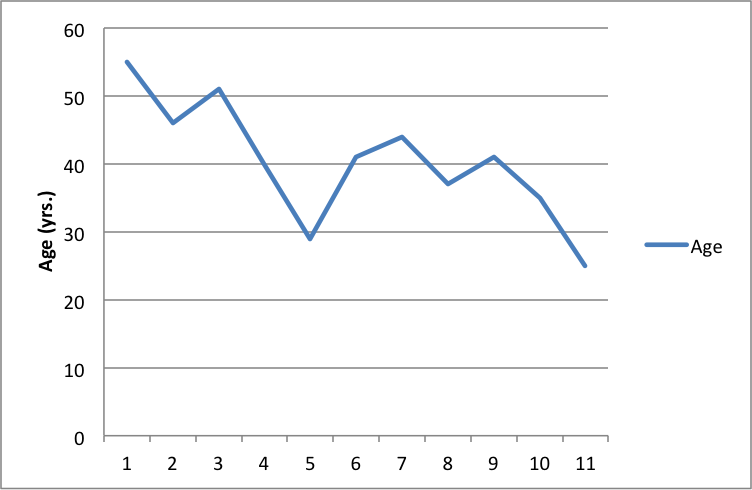
\includegraphics[width=10cm]{./chart-figure-5.png}}
    \caption{This is the figure x1 ทดสอบ จาก \href{https://www.google.com} {https://www.google.com}}\label{fig:x1}
\end{figure}


Explain the motivations of your works.
\begin{itemize}
    \item   What are the problems you are addressing?
    \item  Why they are important?
    \item  What are the limitations of existing approaches?
\end{itemize}
You may combine this section with the background section.



\section{วัตถุประสงค์}

ระบุสิ่งท่ี่จะทำในโครงการ ซึ่งจะใช้สำหรับการประเมินว่าโครงงานทำสำเร็จหรือไม่

\section{ขอบเขตของโครงงาน}

Explain the scope of your works.
\begin{itemize}
    \item   What are the problems you are addressing?
    \item  Why they are important?
    \item  What are the limitations of existing approaches?
\end{itemize}

\section{ประโยชน์ที่คาดว่าจะได้่รับ}

โครงงานนี้จะเป็นประโยชน์กับใคร ยังไง ทั้งในเชิงรูปธรรมและนามธรรม ในปัจจุบันหรือในอนาคตถ้านำไป
ต่อยอด

\section{ตารางการดำเนินงาน}